%fig 11.1
\begin{figure}
\centering
\begin{subfigure}{1\textwidth}
\centering
\begin{tikzpicture}
\pgfmathsetmacro{\klen}{1};
\pgfmathsetmacro{\kpin}{0.5};
\pgfmathsetmacro{\kpina}{0.75};
\pgfmathsetmacro{\ksepX}{1.1}
\pgfmathsetmacro{\ksepY}{2}
\pgfmathsetmacro{\ksepYa}{1.1}
\pgfmathsetmacro{\ksepdX}{0.2}
\draw(0,0)node[and port,scale=1,number inputs=2,scale=1,anchor=out](u0){}  (u0.out)node[right]{$Y$};
\draw(u0.in 2)--++(0,-\kpin)--++(-\kpin,0)node[above]{$\overline{A}$}node[not port,anchor=out,scale=0.8](u1){};
\draw(u0.in 1)--(u0.in 1 -| u1.in)--++(-2*\kpin,0)coordinate(aa)node[left]{$A$};
\draw(u1.in)--++(-\kpin,0)coordinate(bb)--(bb |- aa);
\end{tikzpicture}
\caption{}
\end{subfigure}
\begin{subfigure}{1\textwidth}
\centering
 \begin{tikzpicture}
  \pgfmathsetmacro{\kH}{0.75}
   \pgfmathsetmacro{\ksepY}{\kH+0.5}
\draw[thick](0,0)node[above left]{$A$}--++(2,0)--++(0,\kH)--++(5,0)--++(0,-\kH)--++(2,0);
\draw[thick](0,-\ksepY)node[above left]{$\overline{A}$}  (0,-\ksepY+\kH)--++(3,0)--++(0,-\kH)--++(5,0)--++(0,\kH)--++(1,0);
\draw[thick](0,-2*\ksepY)node[above left]{$Y_0$}--++(2,0)--++(0,\kH)--++(1,0)--++(0,-\kH)--++(6,0);
\draw[thick](0,-3*\ksepY)node[above left]{$Y$}--++(3.25,0)--++(0,\kH)--++(1,0)coordinate[pos=0.5](kglitch)--++(0,-\kH)--++(4.75,0);
\draw[dashed](2,\kH)++(0,0.2)--++(0,0.5)coordinate(aa)  (3,-\ksepY+\kH)++(0,0.2)coordinate(bbN)--(bbN |- aa) coordinate(bb);
\draw[stealth-stealth]($(aa)+(0,-0.2)$)--($(bb)+(0,-0.2)$)coordinate[pos=0.5](ka);
\draw(ka)++(0,0.2) to [out=90,in=0]++(-1,0.5)node[left]{\RL{نفی گیٹ کا دورانیہ رد عمل}};
\draw[dashed](2,-2*\ksepY)++(0,-0.2)--++(0,-\ksepY-0.7)coordinate(cc)  (3.25,-3*\ksepY)++(0,-0.2)coordinate(ddP)--(ddP |- cc)coordinate(dd);
\draw[stealth-stealth]($(cc)+(0,0.2)$)--($(dd)+(0,0.2)$)coordinate[pos=0.5](kb);
\draw(kb)++(0,-0.2) to [out=-90,in=180]++(1,-0.5)node[right]{\RL{ضرب گیٹ کا دورانیہ رد عمل}};
\draw(kglitch)++(0,0.2) to [out=90,in=180]++(0.5,0.75)node[right]{\RL{لرزش}};
\end{tikzpicture}
\caption{}
\end{subfigure}
\end{figure}
%===================
%fig 11.2
\begin{figure}
\centering
\begin{subfigure}{1\textwidth}
\centering
\begin{tikzpicture}
\pgfmathsetmacro{\klen}{1};
\pgfmathsetmacro{\kpin}{0.5};
\pgfmathsetmacro{\kpina}{0.25};
\pgfmathsetmacro{\ksepX}{1.1}
\pgfmathsetmacro{\ksepY}{2}
\pgfmathsetmacro{\ksepYa}{1.1}
\pgfmathsetmacro{\ksepdX}{0.2}
\draw(0,0)node[xor port,number inputs=2,scale=1](u0){};
\path($(u0.in 1)!0.5!(u0.in 2)$)++(0,0.5*\kpina)coordinate(kup);
\draw(u0.out)node[right]{$Y$};
\draw(u0.in 1)--++(0,2*\kpin)coordinate[pos=0.75](kst)node[above]{$A$};
\draw(u0.in 1)--++(-\kpin,0)--++(0,\kpin)--++(-\kpina,0)--++(0,-\kpin)--++(-\kpina,0)--++(0,\kpin)--++(-\kpina,0)--++(0,-\kpin)--++(-\kpina,0)--++(0,\kpin)--++(-\kpina,0)--++(0,-\kpin)--++(-\kpina,0)--++(0,\kpin)--++(-\kpina,0)--++(0,-\kpin)--++(-\kpina,0)--++(0,\kpin)--++(-\kpina,0)--++(0,-\kpin)coordinate(aaa)--(aaa |- kup)--++(-\kpin,0)coordinate(kmid)--++(0,-\kpina)--++(\kpin,0)coordinate(cc)--(cc |- u0.in 2)--++(0,-\kpin)coordinate(kbot)--++(\kpina,0)--++(0,\kpin)--++(\kpina,0)--++(0,-\kpin)--++(\kpina,0)--++(0,\kpin)--++(\kpina,0)--++(0,-\kpin)--++(\kpina,0)--++(0,\kpin)--++(\kpina,0)--++(0,-\kpin)--++(\kpina,0)--++(0,\kpin)--++(\kpina,0)--++(0,-\kpin)--++(\kpina,0)coordinate(kend)--++(0,\kpin)--(u0.in 2)node[below,xshift=-1ex]{$A_t$};
\draw[stealth-stealth](kst)--(kst-| kmid)--++(-1.5*\kpin,0)coordinate(ktop)--(ktop |- kbot)coordinate[pos=0.5](ktxt)--++(0,-0.5*\kpin)coordinate(kklft)--(kklft -| u0.in 2);
\draw(ktxt)node[fill=white,xshift=-0.5cm]{\RL{تیس سنٹی میٹر}};
\end{tikzpicture}
\caption{}
\end{subfigure}
\begin{subfigure}{1\textwidth}
\centering
 \begin{tikzpicture}
  \pgfmathsetmacro{\kH}{0.75}
   \pgfmathsetmacro{\ksepY}{\kH+0.5}
\draw[thick](0,0)node[above left]{$A$}--++(2,0)--++(0,\kH)--++(5,0)--++(0,-\kH)--++(4,0);
\draw[thick](0,-\ksepY)node[above left]{$A_t$}--++(3,0)--++(0,\kH)--++(5,0)--++(0,-\kH)--++(3,0);
\draw[thick](0,-2*\ksepY)node[above left]{$Y_0$}--++(2,0)--++(0,\kH)--++(1,0)--++(0,-\kH)--++(4,0)--++(0,\kH)--++(1,0)--++(0,-\kH)--++(3,0);
\draw[thick](0,-3*\ksepY)node[above left]{$Y$}--++(3.25,0)--++(0,\kH)--++(1,0)coordinate[pos=0.5](kglitch)--++(0,-\kH)--++(4,0)--++(0,\kH)--++(1,0)coordinate[pos=0.5](kglitchA)--++(0,-\kH)--++(1.75,0);
\draw[dashed](2,\kH)++(0,0.2)--++(0,0.5)coordinate(aa)  (3,-\ksepY+\kH)++(0,0.2)coordinate(bbN)--(bbN |- aa) coordinate(bb);
\draw[stealth-stealth]($(aa)+(0,-0.2)$)--($(bb)+(0,-0.2)$)coordinate[pos=0.5](ka);
\draw(ka)++(0,0.2) to [out=90,in=0]++(-1,0.5)node[left]{\RL{ایک نینو سیکنڈ}};
\draw[dashed](2,-2*\ksepY)++(0,-0.2)--++(0,-\ksepY-0.7)coordinate(cc)  (3.25,-3*\ksepY)++(0,-0.2)coordinate(ddP)--(ddP |- cc)coordinate(dd);
\draw[stealth-stealth]($(cc)+(0,0.2)$)--($(dd)+(0,0.2)$)coordinate[pos=0.5](kb);
\draw(kb)++(0,-0.2) to [out=-90,in=180]++(1,-0.5)node[right]{\RL{بلا شرکت جمع  گیٹ کا دورانیہ رد عمل}};
\draw(kglitch)++(0,0.2) to [out=90,in=180]++(0.5,0.75)node[right]{\RL{لرزش}};
\draw(kglitchA)++(0,0.2) to [out=90,in=180]++(0.5,0.75)node[right]{\RL{لرزش}};
\end{tikzpicture}
\caption{}
\end{subfigure}
\end{figure}
%=======================
%fig 11.3
\begin{figure}
\centering
\begin{tikzpicture}
\pgfmathsetmacro{\klen}{1};
\pgfmathsetmacro{\kpin}{0.5};
\pgfmathsetmacro{\kpina}{0.25};
\pgfmathsetmacro{\ksepX}{1.1}
\pgfmathsetmacro{\ksepY}{2}
\pgfmathsetmacro{\ksepYa}{1.1}
\pgfmathsetmacro{\ksepdX}{0.2}
\draw(0,0)node[and port,number inputs=2,scale=1,anchor=out](u0){};
\draw(0,\ksepY)node[and port,number inputs=2,scale=1,anchor=out](u1){};
\draw(u1.in 1)--++(0,\kpin)--++(-\kpin,0)node[or port,scale=1,number inputs=2,anchor=out](u2){};
\draw(u1.in 2)--++(-\kpin,0)--++(0,-\kpin)node[or port,scale=1,anchor=out,number inputs=2](u3){};
\draw(u0.in 2)--++(-\kpin,0)node[or port,scale=1,number inputs=2,anchor=out](u4){};
\draw(u1.in 1)--(u0.in 1);
\draw(u4.in 2)--++(-\kpin,0)node[not port,anchor=out,scale=0.8](u5){};
\draw(u3.in 1)--++(-\kpin,0)node[not port,anchor=out,scale=0.8](u6){};
\draw(u6.out)|-(u4.in 1);
\draw(u3.in 2)--++(0,-\kpin)-|(u5.in)node[left]{$a$} --++(0,-2*\kpin)-|(u1.out)--++(\kpin,0)node[right]{$A$};
\draw(u0.out)--++(\kpin,0)coordinate[pos=0.5](kB)node[right]{$B$};
\draw(u2.in 1)node[above left]{$b$}--++(0,2*\kpin)-|(kB);
\draw(u2.in 2)--(u2.in 2-| u5.in)--++(-\kpin,0)node[left]{$X$};
\draw(u6.in)--(u6.in |- u2.in 2);
\end{tikzpicture}
\caption{}
\end{figure}
%===================
%fig 11.4
\begin{figure}
\centering
\begin{tikzpicture}
\pgfmathsetmacro{\kxstep}{1}
\pgfmathsetmacro{\kystep}{1}
\pgfmathsetmacro{\kpin}{0.75}
\pgfmathsetmacro{\ksepX}{2*\kxstep+2}
\draw[xstep=\kxstep,ystep=\kystep](0,0) grid ++(2*\kxstep,-4*\kystep);
\draw(0,0)--++(135:\kpin)node[pos=0.75,above right]{$x$}node[pos=0.75,below left]{$ab$};
\foreach \kx/\xlb in {0/{0},1/{1}}{\draw(\kx*\kxstep+\kxstep/2,0)node[above]{$\xlb$};}
\foreach \ky/\ylb in {0/{00},1/{01},2/{11},3/{10}}{\draw(0,-\ky*\kystep-\kystep/2)node[left]{$\ylb$};}
\foreach \kx/\xlb in {0/0,1/0}{\draw(\kx*\kxstep+\kxstep/2,-\kystep/2)node[]{$\xlb$};}
\foreach \kx/\xlb in {0/1,1/0}{\draw(\kx*\kxstep+\kxstep/2,-1.5*\kystep)node[]{$\xlb$};}
\foreach \kx/\xlb in {0/1,1/1}{\draw(\kx*\kxstep+\kxstep/2,-2.5*\kystep)node[]{$\xlb$};}
\foreach \kx/\xlb in {0/0,1/1}{\draw(\kx*\kxstep+\kxstep/2,-3.5*\kystep)node[]{$\xlb$};}
\draw[xstep=\kxstep,ystep=\kystep](\ksepX,0) grid ++(2*\kxstep,-4*\kystep);
\draw(\ksepX,0)--++(135:\kpin)node[pos=0.75,above right]{$x$}node[pos=0.75,below left]{$ab$};
\foreach \kx/\xlb in {0/{0},1/{1}}{\draw(\ksepX+\kx*\kxstep+\kxstep/2,0)node[above]{$\xlb$};}
\foreach \ky/\ylb in {0/{00},1/{01},2/{11},3/{10}}{\draw(\ksepX,-\ky*\kystep-\kystep/2)node[left]{$\ylb$};}
\foreach \kx/\xlb in {0/0,1/1}{\draw(\ksepX+\kx*\kxstep+\kxstep/2,-\kystep/2)node[]{$\xlb$};}
\foreach \kx/\xlb in {0/1,1/1}{\draw(\ksepX+\kx*\kxstep+\kxstep/2,-1.5*\kystep)node[]{$\xlb$};}
\foreach \kx/\xlb in {0/1,1/0}{\draw(\ksepX+\kx*\kxstep+\kxstep/2,-2.5*\kystep)node[]{$\xlb$};}
\foreach \kx/\xlb in {0/0,1/0}{\draw(\ksepX+\kx*\kxstep+\kxstep/2,-3.5*\kystep)node[]{$\xlb$};}
\draw[xstep=\kxstep,ystep=\kystep](2*\ksepX,0) grid ++(2*\kxstep,-4*\kystep);
\draw(2*\ksepX,0)--++(135:\kpin)node[pos=0.75,above right]{$x$}node[pos=0.75,below left]{$ab$};
\foreach \kx/\xlb in {0/{0},1/{1}}{\draw(2*\ksepX+\kx*\kxstep+\kxstep/2,0)node[above]{$\xlb$};}
\foreach \ky/\ylb in {0/{00},1/{01},2/{11},3/{10}}{\draw(2*\ksepX,-\ky*\kystep-\kystep/2)node[left]{$\ylb$};}
\foreach \kx/\xlb in {0/00,1/01}{\draw(2*\ksepX+\kx*\kxstep+\kxstep/2,-\kystep/2)node[]{$\xlb$};}
\foreach \kx/\xlb in {0/11,1/01}{\draw(2*\ksepX+\kx*\kxstep+\kxstep/2,-1.5*\kystep)node[]{$\xlb$};}
\foreach \kx/\xlb in {0/11,1/10}{\draw(2*\ksepX+\kx*\kxstep+\kxstep/2,-2.5*\kystep)node[]{$\xlb$};}
\foreach \kx/\xlb in {0/00,1/10}{\draw(2*\ksepX+\kx*\kxstep+\kxstep/2,-3.5*\kystep)node[]{$\xlb$};}
\draw(2*\ksepX+0*\kxstep+\kxstep/2,-\kystep/2)node[draw,circle,inner sep=1pt]{$\phantom{00}$};
\draw(2*\ksepX+1*\kxstep+\kxstep/2,-\kystep-\kystep/2)node[draw,circle,inner sep=1pt]{$\phantom{00}$};
\draw(2*\ksepX+0*\kxstep+\kxstep/2,-2*\kystep-\kystep/2)node[draw,circle,inner sep=1pt]{$\phantom{00}$};
\draw(2*\ksepX+1*\kxstep+\kxstep/2,-3*\kystep-\kystep/2)coordinate(kend)node[draw,circle,inner sep=1pt]{$\phantom{00}$};
\draw[-stealth](0*\ksepX+1*\kxstep+\kxstep/2,-3*\kystep-\kystep/2)++(0.2,-0.2) to [out=-10,in=-135] ($(kend)+(-0.2,-0.2)$); 
\draw[-stealth](1*\ksepX+1*\kxstep+\kxstep/2,-3*\kystep-\kystep/2)++(0.2,-0.2) to [out=-45,in=-90] ($(kend)+(0.1,-0.25)$); 
\draw(0*\ksepX+1*\kxstep,-5*\kystep)node[below]{$A=(b+x)(a+\overline{x})$};
\draw(1*\ksepX+1*\kxstep,-5*\kystep)node[below]{$B=(b+x)(\overline{a}+\overline{x})$};
\draw(0*\ksepX+1*\kxstep,1*\kystep)node[above]{\RL{کارناف نقشہ برائے \عددی{A}}};
\draw(1*\ksepX+1*\kxstep,1*\kystep)node[above]{\RL{کارناف  نقشہ برائے \عددی{B}}};
\draw(2*\ksepX+1*\kxstep,1*\kystep)node[above]{\RL{عبوری جدول}};
\end{tikzpicture}
\end{figure}
%===================
%fig 11.5
\begin{figure}
\centering
\begin{tikzpicture}
\pgfmathsetmacro{\kxstep}{1}
\pgfmathsetmacro{\kystep}{1}
\pgfmathsetmacro{\kpin}{0.75}
\pgfmathsetmacro{\ksepX}{2*\kxstep+2}
\draw[xstep=\kxstep,ystep=\kystep](0,0) grid ++(2*\kxstep,-4*\kystep);
\draw(0,0)--++(135:\kpin)node[pos=0.75,above right]{$x$}node[pos=0.75,below left]{$ab$};
\foreach \kx/\xlb in {0/{0},1/{1}}{\draw(\kx*\kxstep+\kxstep/2,0)node[above]{$\xlb$};}
\foreach \ky/\ylb in {0/{00},1/{01},2/{11},3/{10}}{\draw(0,-\ky*\kystep-\kystep/2)node[left]{$\ylb$};}
\foreach \kx/\xlb in {0/00,1/01}{\draw(\kx*\kxstep+\kxstep/2,-\kystep/2)node[]{$\xlb$};}
\foreach \kx/\xlb in {0/11,1/01}{\draw(\kx*\kxstep+\kxstep/2,-1.5*\kystep)node[]{$\xlb$};}
\foreach \kx/\xlb in {0/11,1/10}{\draw(\kx*\kxstep+\kxstep/2,-2.5*\kystep)node[]{$\xlb$};}
\foreach \kx/\xlb in {0/00,1/10}{\draw(\kx*\kxstep+\kxstep/2,-3.5*\kystep)node[]{$\xlb$};}
\draw(0*\kxstep+\kxstep/2,-\kystep/2)node[draw,circle,inner sep=1pt](ka){$\phantom{00}$};
\draw(1*\kxstep+\kxstep/2,-\kystep-\kystep/2)node[draw,circle,inner sep=1pt](kb){$\phantom{00}$};
\draw(0*\kxstep+\kxstep/2,-2*\kystep-\kystep/2)node[draw,circle,inner sep=1pt](kc){$\phantom{00}$};
\draw(1*\kxstep+\kxstep/2,-3*\kystep-\kystep/2)coordinate(kend)node[draw,circle,inner sep=1pt](kd){$\phantom{00}$};
\draw[-stealth,very thick](ka.0) to [out=0,in=90] (kb.90);
\draw[-stealth](kb.180) to [out=180,in=90] (kc.90);
\draw[-stealth](kc.0) to [out=0,in=90] (kd.90);
\draw[-stealth](kd.0) to [out=0,in=-90]  (3*\kxstep,-2*\kystep) to [out=90,in=90](ka.90);
\draw(ka.-150)++(-0.1,-0.1) to [out=-150,in=0]++(-1,-0.5)node[left]{\RL{ابتدائی خانہ}};
\end{tikzpicture}
\end{figure}
%===================
%fig 11.6
\begin{figure}
\centering
\begin{tikzpicture}
\pgfmathsetmacro{\kxstep}{1}
\pgfmathsetmacro{\kystep}{1}
\pgfmathsetmacro{\kpin}{0.75}
\pgfmathsetmacro{\ksepX}{2*\kxstep+2}
\draw[xstep=\kxstep,ystep=\kystep](0,0) grid ++(2*\kxstep,-4*\kystep);
\draw(0,0)--++(135:\kpin)node[pos=0.75,above right]{$x$}node[pos=0.75,below left]{$ab$};
\foreach \kx/\xlb in {0/{0},1/{1}}{\draw(\kx*\kxstep+\kxstep/2,0)node[above]{$\xlb$};}
\foreach \ky/\ylb in {0/{00},1/{01},2/{11},3/{10}}{\draw(0,-\ky*\kystep-\kystep/2)node[left]{$\ylb$};}
\foreach \kx/\xlb in {0/00,1/01}{\draw(\kx*\kxstep+\kxstep/2,-\kystep/2)node[]{$\xlb$};}
\foreach \kx/\xlb in {0/11,1/01}{\draw(\kx*\kxstep+\kxstep/2,-1.5*\kystep)node[]{$\xlb$};}
\foreach \kx/\xlb in {0/11,1/10}{\draw(\kx*\kxstep+\kxstep/2,-2.5*\kystep)node[]{$\xlb$};}
\foreach \kx/\xlb in {0/00,1/10}{\draw(\kx*\kxstep+\kxstep/2,-3.5*\kystep)node[]{$\xlb$};}
\draw(0*\kxstep+\kxstep/2,-\kystep/2)node[draw,circle,inner sep=1pt](ka){$\phantom{00}$};
\draw(1*\kxstep+\kxstep/2,-\kystep-\kystep/2)node[draw,circle,inner sep=1pt](kb){$\phantom{00}$};
\draw(0*\kxstep+\kxstep/2,-2*\kystep-\kystep/2)node[draw,circle,inner sep=1pt](kc){$\phantom{00}$};
\draw(1*\kxstep+\kxstep/2,-3*\kystep-\kystep/2)coordinate(kend)node[draw,circle,inner sep=1pt](kd){$\phantom{00}$};
\draw(1*\kxstep,-4*\kystep)node[below]{\RL{عبوری جدول}};
\draw[xstep=\kxstep,ystep=\kystep](2*\ksepX,0) grid ++(2*\kxstep,-4*\kystep);
\draw(2*\ksepX,0)--++(135:\kpin)node[pos=0.75,above right]{$x$}node[pos=0.75,below left]{$ab$};
\foreach \kx/\xlb in {0/{0},1/{1}}{\draw(2*\ksepX+\kx*\kxstep+\kxstep/2,0)node[above]{$\xlb$};}
\foreach \ky/\ylb in {0/{a},1/{b},2/{d},3/{c}}{\draw(2*\ksepX,-\ky*\kystep-\kystep/2)node[left]{$\ylb$};}
\foreach \kx/\xlb in {0/a,1/b}{\draw(2*\ksepX+\kx*\kxstep+\kxstep/2,-\kystep/2)node[]{$\xlb$};}
\foreach \kx/\xlb in {0/d,1/b}{\draw(2*\ksepX+\kx*\kxstep+\kxstep/2,-1.5*\kystep)node[]{$\xlb$};}
\foreach \kx/\xlb in {0/d,1/c}{\draw(2*\ksepX+\kx*\kxstep+\kxstep/2,-2.5*\kystep)node[]{$\xlb$};}
\foreach \kx/\xlb in {0/a,1/c}{\draw(2*\ksepX+\kx*\kxstep+\kxstep/2,-3.5*\kystep)node[]{$\xlb$};}
\draw(2*\ksepX+0*\kxstep+\kxstep/2,-\kystep/2)node[draw,circle,inner sep=1pt](ka){$\phantom{00}$};
\draw(2*\ksepX+1*\kxstep+\kxstep/2,-\kystep-\kystep/2)node[draw,circle,inner sep=1pt](kb){$\phantom{00}$};
\draw(2*\ksepX+0*\kxstep+\kxstep/2,-2*\kystep-\kystep/2)node[draw,circle,inner sep=1pt](kc){$\phantom{00}$};
\draw(2*\ksepX+1*\kxstep+\kxstep/2,-3*\kystep-\kystep/2)coordinate(kend)node[draw,circle,inner sep=1pt](kd){$\phantom{00}$};
\draw(2*\ksepX+1*\kxstep,-4*\kystep)node[below]{\RL{جدول بہاو}};
\draw(\ksepX+\kxstep,0)node[below]{$\begin{aligned} 00&=a\\  01&=b\\ 10&=c\\ 11&=d \end{aligned}$};
\end{tikzpicture}
\end{figure}
%===================
%fig 11.7
\begin{figure}
\centering
\begin{tikzpicture}
\pgfmathsetmacro{\kxstep}{0.75}
\pgfmathsetmacro{\kystep}{0.75}
\pgfmathsetmacro{\kpin}{0.75}
\pgfmathsetmacro{\ksepX}{2*\kxstep+2}
\foreach \x in {0,1,2,3,4}{\draw(\x*\kxstep,0)--++(0,-2*\kystep);}
\foreach \x in {0,1,2}{\draw(0,-\x*\kystep)--++(4*\kxstep,0);}
\draw(0,0)--++(135:\kpin)node[pos=0.75,above right]{$x_1x_0$}node[pos=0.75,below left]{$y$};
\foreach \kx/\xlb in {0/{00},1/{01},2/11,3/10}{\draw(\kx*\kxstep+\kxstep/2,0)node[above]{$\xlb$};}
\foreach \ky/\ylb in {0/a,1/b}{\draw(0,-\ky*\kystep-\kystep/2)node[left]{$\ylb$};}
\foreach \kx/\xlb in {0/a,1/b,2/a,3/a}{\draw(\kx*\kxstep+\kxstep/2,-\kystep/2)node[]{$\xlb$};}
\foreach \kx/\xlb in {0/a,1/b,2/b,3/b}{\draw(\kx*\kxstep+\kxstep/2,-1.5*\kystep)node[]{$\xlb$};}
\draw(2*\kxstep,-2*\kystep)node[below]{\RL{بہاو کا جدول}};
\foreach \kx in {0,2,3}{\draw(\kx*\kxstep+\kxstep/2,-\kystep/2)node[draw,circle,inner sep=1pt]{$\phantom{00}$};}
\foreach \kx in {1,2,3}{\draw(\kx*\kxstep+\kxstep/2,-\kystep-\kystep/2)node[draw,circle,inner sep=1pt]{$\phantom{00}$};}

\foreach \x in {0,1,2,3,4}{\draw(2*\ksepX+\x*\kxstep,0)--++(0,-2*\kystep);}
\foreach \x in {0,1,2}{\draw(2*\ksepX,-\x*\kystep)--++(4*\kxstep,0);}

\draw(2*\ksepX,0)--++(135:\kpin)node[pos=0.75,above right]{$x_1x_0$}node[pos=0.75,below left]{$y$};
\foreach \kx/\xlb in {0/{00},1/{01},2/11,3/10}{\draw(2*\ksepX+\kx*\kxstep+\kxstep/2,0)node[above]{$\xlb$};}
\foreach \ky/\ylb in {0/a,1/b}{\draw(2*\ksepX,-\ky*\kystep-\kystep/2)node[left]{$\ylb$};}
\foreach \kx/\xlb in {0/0,1/1,2/0,3/0}{\draw(2*\ksepX+\kx*\kxstep+\kxstep/2,-\kystep/2)node[]{$\xlb$};}
\foreach \kx/\xlb in {0/0,1/1,2/1,3/1}{\draw(2*\ksepX+\kx*\kxstep+\kxstep/2,-1.5*\kystep)node[]{$\xlb$};}
\draw(2*\ksepX+2*\kxstep,-2*\kystep)node[below]{\RL{عبوری جدول}};
\foreach \kx in {0,2,3}{\draw(2*\ksepX+\kx*\kxstep+\kxstep/2,-\kystep/2)node[draw,circle,inner sep=1pt]{$\phantom{00}$};}
\foreach \kx in {1,2,3}{\draw(2*\ksepX+\kx*\kxstep+\kxstep/2,-\kystep-\kystep/2)node[draw,circle,inner sep=1pt]{$\phantom{00}$};}
\draw(\ksepX+2*\kxstep,0)node[below]{$\begin{aligned} a&=0\\ b&=1  \end{aligned}$};
\end{tikzpicture}
\end{figure}
%=====================
%===================
%fig 11.8
\begin{figure}
\centering
\begin{tikzpicture}
\pgfmathsetmacro{\kxstep}{0.75}
\pgfmathsetmacro{\kystep}{0.75}
\pgfmathsetmacro{\kpin}{0.5}
\pgfmathsetmacro{\kpina}{0.75}
\pgfmathsetmacro{\ksepX}{2*\kxstep+2}
\draw(0,0)node[or port,scale=1,number inputs=2,anchor=out](u0){};
\draw(u0.in 2)--++(0,-\kpin)node[and port,scale=1,number inputs=2,anchor=out](u1){};
\draw(u0.in 1)--++(0,\kpin)node[and port,scale=1,number inputs=2,anchor=out](u2){};
\draw(u1.in 1) node[not port,scale=0.8,anchor=out](u3){};
\draw(u2.in 2)--(u2.in 2 -|u3.in)--++(-\kpin,0)coordinate(klft)node[left]{$X_1$};
\draw(u1.in 2)--++(0,-\kpin)coordinate(aa)--(aa -| klft)node[left]{$X_0$};
\draw(u2.in 1)node[left]{$y$}--++(0,\kpin)-|(u0.out)--++(\kpin,0)node[right]{$Y$};
\draw(u3.in)--(u3.in |- klft);
\end{tikzpicture}
\end{figure}
%============================
%fig 11.9
\begin{figure}
\centering
\begin{tikzpicture}
\pgfmathsetmacro{\kxstep}{1}
\pgfmathsetmacro{\kystep}{1}
\pgfmathsetmacro{\kpin}{0.75}
\def\ka{a}
\def\kb{b}
\pgfmathsetmacro{\ksepX}{2*\kxstep+2}
\foreach \x in {0,1,2,3,4}{\draw(\x*\kxstep,0)--++(0,-2*\kystep);}
\foreach \x in {0,1,2}{\draw(0,-\x*\kystep)--++(4*\kxstep,0);}
\draw(0,0)--++(135:\kpin)node[pos=0.75,above right]{$x_1x_0$}node[pos=0.75,below left]{$y$};
\foreach \kx/\xlb in {0/{00},1/{01},2/11,3/10}{\draw(\kx*\kxstep+\kxstep/2,0)node[above]{$\xlb$};}
\foreach \ky/\ylb in {0/a,1/b}{\draw(0,-\ky*\kystep-\kystep/2)node[left]{$\ylb$};}
\foreach \kx/\xlb in {0/a,1/b,2/a,3/a}{\draw(\kx*\kxstep+\kxstep/2,-\kystep/2)node[]{$\xlb$};}
\foreach \kx/\xlb in {0/a,1/b,2/b,3/b}{\draw(\kx*\kxstep+\kxstep/2,-1.5*\kystep)node[]{$\xlb$};}
\foreach \kx in {0,2,3}{\draw(\kx*\kxstep+\kxstep/2,-\kystep/2)node[draw,circle,inner sep=1pt]{$\phantom{00}$};}
\foreach \kx in {1,2,3}{\draw(\kx*\kxstep+\kxstep/2,-\kystep-\kystep/2)node[draw,circle,inner sep=1pt]{$\phantom{00}$};}
\foreach \kx in {0,1,2,3}{\path(\kx*\kxstep+\kxstep/2,-\kystep/2)node[draw,circle,inner sep=1pt](\ka\kx){$\phantom{00}$};}
\foreach \kx in {0,1,2,3}{\path(\kx*\kxstep+\kxstep/2,-\kystep-\kystep/2)node[draw,circle,inner sep=1pt](\kb\kx){$\phantom{00}$};}
\draw[-stealth,thick](a0.0) to [out=0,in=90] (b1.90);
\draw[-stealth](b1.0) to [out=0,in=180] (b2.180);
\draw[-stealth,thick](a0.70) to [out=70,in=110](a3.110);
\draw[-stealth](a3.180)--(a2.0);
\draw(a0.180)++(-0.1,0) to [out=135,in=0]++(-1.5,0.25)node[left]{\RL{ابتدائی خانہ}};
\draw(b2.-90)++(0,-0.1) to [out=-90,in=180]++(0.5,-0.5)node[right]{\RL{پہلا اختتام}};
\draw(a2.-45)++(0.1,-0.1) to [out=-45,in=180]++(1.5,-0.35)node[right]{\RL{دوسرا اختتام}};
\end{tikzpicture}
\end{figure}
%============
%============================
%fig 11.10
\begin{figure}
\centering
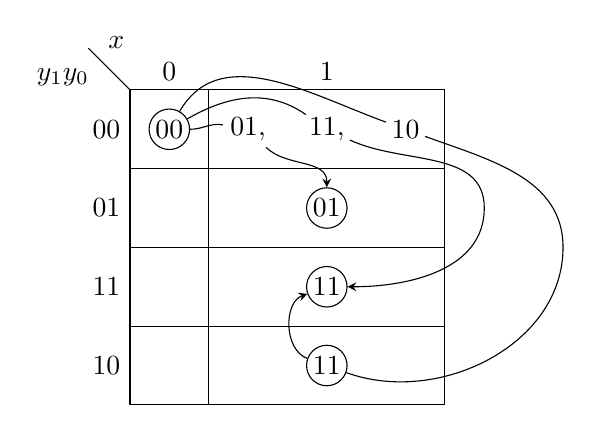
\begin{tikzpicture}
\pgfmathsetmacro{\kxstep}{1}
\pgfmathsetmacro{\kystep}{1}
\pgfmathsetmacro{\kpin}{0.75}
\def\ka{a}
\def\kb{b}
\pgfmathsetmacro{\ksepX}{2*\kxstep+2}
\foreach \x in {0,1,4}{\draw(\x*\kxstep,0)--++(0,-4*\kystep);}
\foreach \x in {0,1,2,3,4}{\draw(0,-\x*\kystep)--++(4*\kxstep,0);}
\draw(0,0)--++(135:\kpin)node[pos=0.75,above right]{$x$}node[pos=0.75,below left]{$y_1y_0$};
\foreach \kx/\xlb in {0/{0},2/{1}}{\draw(\kx*\kxstep+\kxstep/2,0)node[above]{$\xlb$};}
\foreach \ky/\ylb in {0/00,1/01,2/11,3/10}{\draw(0,-\ky*\kystep-\kystep/2)node[left]{$\ylb$};}
\draw(0.5*\kxstep,-0.5*\kystep)node[draw,circle,inner sep=1pt](a0){$00$};
\draw(1.5*\kxstep,-0.5*\kystep)node[,circle,inner sep=1pt](a1){$01,$};
\draw(2.5*\kxstep,-0.5*\kystep)node[,circle,inner sep=1pt](a2){$11,$};
\draw(3.5*\kxstep,-0.5*\kystep)node[,circle,inner sep=1pt](a3){$10$};
\draw(2.5*\kxstep,-1.5*\kystep)node[draw,circle,inner sep=1pt](b2){$01$};
\draw(2.5*\kxstep,-2.5*\kystep)node[draw,circle,inner sep=1pt](c2){$11$};
\draw(2.5*\kxstep,-3.5*\kystep)node[draw,circle,inner sep=1pt](d2){$11$};
\draw[-stealth](a0.0) to [out=0,in=170] (a1) to [out=-45,in=90] (b2.90);
\draw[-stealth](a0.30) to [out=30,in=145](a2) to [out=-25,in=90] (4.5*\kxstep,-1.5*\kystep) to [out=-90,in=0] (c2.0);
\draw[-stealth](a0.60) to [out=60,in=160](a3) to [out=-20,in=90] (5.5*\kxstep,-2*\kystep) to [out=-90,in=-20] (d2) to [out=160,in=-160] (c2);
\end{tikzpicture}
\end{figure}
%============
%fig 11.11
\begin{figure}
\centering
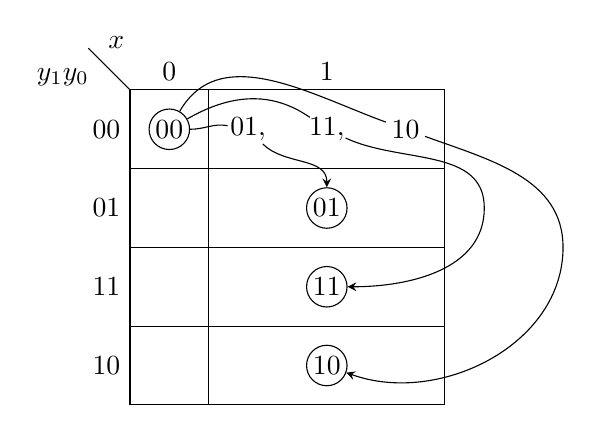
\begin{tikzpicture}
\pgfmathsetmacro{\kxstep}{1}
\pgfmathsetmacro{\kystep}{1}
\pgfmathsetmacro{\kpin}{0.75}
\def\ka{a}
\def\kb{b}
\pgfmathsetmacro{\ksepX}{2*\kxstep+2}
\foreach \x in {0,1,4}{\draw(\x*\kxstep,0)--++(0,-4*\kystep);}
\foreach \x in {0,1,2,3,4}{\draw(0,-\x*\kystep)--++(4*\kxstep,0);}
\draw(0,0)--++(135:\kpin)node[pos=0.75,above right]{$x$}node[pos=0.75,below left]{$y_1y_0$};
\foreach \kx/\xlb in {0/{0},2/{1}}{\draw(\kx*\kxstep+\kxstep/2,0)node[above]{$\xlb$};}
\foreach \ky/\ylb in {0/00,1/01,2/11,3/10}{\draw(0,-\ky*\kystep-\kystep/2)node[left]{$\ylb$};}
\foreach \kx/\a in {0/{00},1/{01,},2/{11,},3/{10}}{\draw(\kx*\kxstep+0.5*\kxstep,-0.5*\kystep)node[]{$\a$};}
\foreach \kx/\a in {2/01}{\draw(\kx*\kxstep+0.5*\kxstep,-1.5*\kystep)node[circle,inner sep=1pt](b\kx){$\a$};}
\foreach \kx/\a in {2/11}{\draw(\kx*\kxstep+0.5*\kxstep,-2.5*\kystep)node[circle,inner sep=1pt](c\kx){$\a$};}
\foreach \kx/\a in {2/10}{\draw(\kx*\kxstep+0.5*\kxstep,-3.5*\kystep)node[circle,inner sep=1pt](d\kx){$\a$};}
\foreach \kx in {0,1,2,3}{\draw(\kx*\kxstep+0.5*\kxstep,-0.5*\kystep)node[circle,inner sep=1pt](a\kx){$\phantom{00}$};}
\foreach \kx in {0,1,2,3}{\draw(\kx*\kxstep+0.5*\kxstep,-1.5*\kystep)node[circle,inner sep=1pt](b\kx){$\phantom{00}$};}
\foreach \kx in {0,1,2,3}{\draw(\kx*\kxstep+0.5*\kxstep,-2.5*\kystep)node[circle,inner sep=1pt](c\kx){$\phantom{00}$};}
\foreach \kx in {0,1,2,3}{\draw(\kx*\kxstep+0.5*\kxstep,-3.5*\kystep)node[circle,inner sep=1pt](d\kx){$\phantom{00}$};}
\foreach \kx in {0}{\draw(\kx*\kxstep+0.5*\kxstep,-0.5*\kystep)node[draw,circle,inner sep=1pt]{$\phantom{00}$};}
\foreach \kx in {2}{\draw(\kx*\kxstep+0.5*\kxstep,-1.5*\kystep)node[draw,circle,inner sep=1pt]{$\phantom{00}$};}
\foreach \kx in {2}{\draw(\kx*\kxstep+0.5*\kxstep,-2.5*\kystep)node[draw,circle,inner sep=1pt]{$\phantom{00}$};}
\foreach \kx in {2}{\draw(\kx*\kxstep+0.5*\kxstep,-3.5*\kystep)node[draw,circle,inner sep=1pt]{$\phantom{00}$};}
\draw[-stealth](a0.0) to [out=0,in=170] (a1) to [out=-45,in=90] (b2.90);
\draw[-stealth](a0.30) to [out=30,in=145](a2) to [out=-25,in=90] (4.5*\kxstep,-1.5*\kystep) to [out=-90,in=0] (c2.0);
\draw[-stealth](a0.60) to [out=60,in=160](a3) to [out=-20,in=90] (5.5*\kxstep,-2*\kystep) to [out=-90,in=-20] (d2);
\end{tikzpicture}
\end{figure}
%============
%============
%fig 11.12
\begin{figure}
\centering
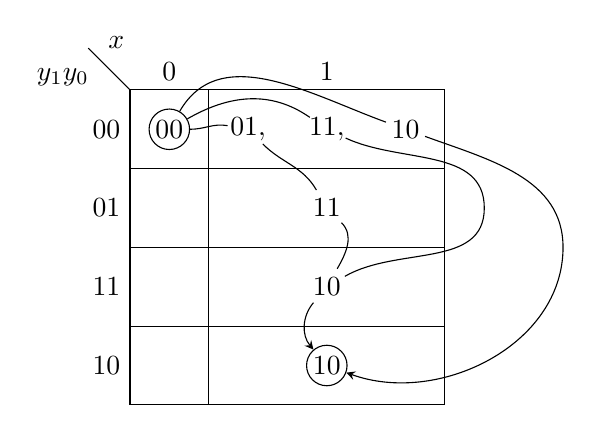
\begin{tikzpicture}
\pgfmathsetmacro{\kxstep}{1}
\pgfmathsetmacro{\kystep}{1}
\pgfmathsetmacro{\kpin}{0.75}
\def\ka{a}
\def\kb{b}
\pgfmathsetmacro{\ksepX}{2*\kxstep+2}
\foreach \x in {0,1,4}{\draw(\x*\kxstep,0)--++(0,-4*\kystep);}
\foreach \x in {0,1,2,3,4}{\draw(0,-\x*\kystep)--++(4*\kxstep,0);}
\draw(0,0)--++(135:\kpin)node[pos=0.75,above right]{$x$}node[pos=0.75,below left]{$y_1y_0$};
\foreach \kx/\xlb in {0/{0},2/{1}}{\draw(\kx*\kxstep+\kxstep/2,0)node[above]{$\xlb$};}
\foreach \ky/\ylb in {0/00,1/01,2/11,3/10}{\draw(0,-\ky*\kystep-\kystep/2)node[left]{$\ylb$};}
\foreach \kx/\a in {0/{00},1/{01,},2/{11,},3/{10}}{\draw(\kx*\kxstep+0.5*\kxstep,-0.5*\kystep)node[]{$\a$};}
\foreach \kx/\a in {2/11}{\draw(\kx*\kxstep+0.5*\kxstep,-1.5*\kystep)node{$\a$};}
\foreach \kx/\a in {2/10}{\draw(\kx*\kxstep+0.5*\kxstep,-2.5*\kystep)node{$\a$};}
\foreach \kx/\a in {2/10}{\draw(\kx*\kxstep+0.5*\kxstep,-3.5*\kystep)node{$\a$};}
\foreach \kx in {0,1,2,3}{\draw(\kx*\kxstep+0.5*\kxstep,-0.5*\kystep)node[circle,inner sep=1pt](a\kx){$\phantom{00}$};}
\foreach \kx in {0,1,2,3}{\draw(\kx*\kxstep+0.5*\kxstep,-1.5*\kystep)node[circle,inner sep=1pt](b\kx){$\phantom{00}$};}
\foreach \kx in {0,1,2,3}{\draw(\kx*\kxstep+0.5*\kxstep,-2.5*\kystep)node[circle,inner sep=1pt](c\kx){$\phantom{00}$};}
\foreach \kx in {0,1,2,3}{\draw(\kx*\kxstep+0.5*\kxstep,-3.5*\kystep)node[circle,inner sep=1pt](d\kx){$\phantom{00}$};}
\foreach \kx in {0}{\draw(\kx*\kxstep+0.5*\kxstep,-0.5*\kystep)node[draw,circle,inner sep=1pt]{$\phantom{00}$};}
%\foreach \kx in {2}{\draw(\kx*\kxstep+0.5*\kxstep,-1.5*\kystep)node[draw,circle,inner sep=1pt]{$\phantom{00}$};}
%\foreach \kx in {2}{\draw(\kx*\kxstep+0.5*\kxstep,-2.5*\kystep)node[draw,circle,inner sep=1pt]{$\phantom{00}$};}
\foreach \kx in {2}{\draw(\kx*\kxstep+0.5*\kxstep,-3.5*\kystep)node[draw,circle,inner sep=1pt]{$\phantom{00}$};}
\draw[](a0) to [out=0,in=170] (a1) to [out=-45,in=120] (b2) to [out=-45,in=60](c2);
\draw[-stealth](a0) to [out=30,in=145](a2) to [out=-25,in=90] (4.5*\kxstep,-1.5*\kystep) to [out=-90,in=30] (c2) to [out=-130,in=130] (d2);
\draw[-stealth](a0) to [out=60,in=160](a3) to [out=-20,in=90] (5.5*\kxstep,-2*\kystep) to [out=-90,in=-20] (d2);
\end{tikzpicture}
\end{figure}
%============
%fig 11.13
\begin{figure}
\centering
\begin{subfigure}{0.45\textwidth}
\centering
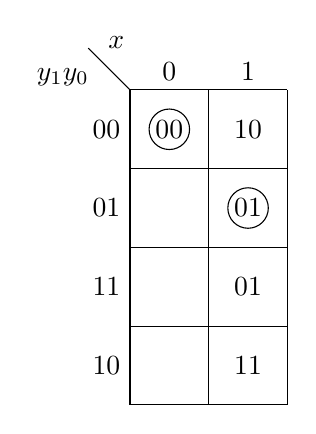
\begin{tikzpicture}
\pgfmathsetmacro{\kxstep}{1}
\pgfmathsetmacro{\kystep}{1}
\pgfmathsetmacro{\kpin}{0.75}
\def\ka{a}
\def\kb{b}
\pgfmathsetmacro{\ksepX}{2*\kxstep+2}
\foreach \x in {0,1,2}{\draw(\x*\kxstep,0)--++(0,-4*\kystep);}
\foreach \x in {0,1,2,3,4}{\draw(0,-\x*\kystep)--++(2*\kxstep,0);}
\draw(0,0)--++(135:\kpin)node[pos=0.75,above right]{$x$}node[pos=0.75,below left]{$y_1y_0$};
\foreach \kx/\xlb in {0/{0},1/{1}}{\draw(\kx*\kxstep+\kxstep/2,0)node[above]{$\xlb$};}
\foreach \ky/\ylb in {0/00,1/01,2/11,3/10}{\draw(0,-\ky*\kystep-\kystep/2)node[left]{$\ylb$};}
\foreach \kx/\a in {0/00,1/10}{\draw(\kx*\kxstep+0.5*\kxstep,-0.5*\kystep)node[]{$\a$};}
\foreach \kx/\a in {1/01}{\draw(\kx*\kxstep+0.5*\kxstep,-1.5*\kystep)node{$\a$};}
\foreach \kx/\a in {1/01}{\draw(\kx*\kxstep+0.5*\kxstep,-2.5*\kystep)node{$\a$};}
\foreach \kx/\a in {1/11}{\draw(\kx*\kxstep+0.5*\kxstep,-3.5*\kystep)node{$\a$};}
\foreach \kx in {0}{\draw(\kx*\kxstep+0.5*\kxstep,-0.5*\kystep)node[draw,circle,inner sep=1pt]{$\phantom{00}$};}
\foreach \kx in {1}{\draw(\kx*\kxstep+0.5*\kxstep,-1.5*\kystep)node[draw,circle,inner sep=1pt]{$\phantom{00}$};}
%\foreach \kx in {1}{\draw(\kx*\kxstep+0.5*\kxstep,-2.5*\kystep)node[draw,circle,inner sep=1pt]{$\phantom{00}$};}
%\foreach \kx in {1}{\draw(\kx*\kxstep+0.5*\kxstep,-3.5*\kystep)node[draw,circle,inner sep=1pt]{$\phantom{00}$};}
\end{tikzpicture}
\caption{}
\end{subfigure}\hfill
\begin{subfigure}{0.45\textwidth}
\centering
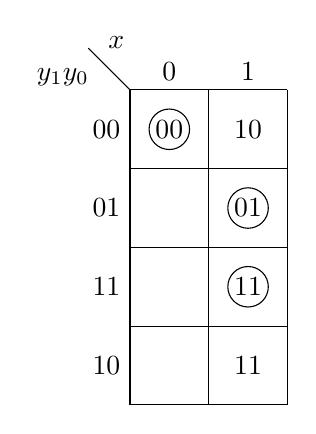
\begin{tikzpicture}
\pgfmathsetmacro{\kxstep}{1}
\pgfmathsetmacro{\kystep}{1}
\pgfmathsetmacro{\kpin}{0.75}
\def\ka{a}
\def\kb{b}
\pgfmathsetmacro{\ksepX}{2*\kxstep+2}
\foreach \x in {0,1,2}{\draw(\x*\kxstep,0)--++(0,-4*\kystep);}
\foreach \x in {0,1,2,3,4}{\draw(0,-\x*\kystep)--++(2*\kxstep,0);}
\draw(0,0)--++(135:\kpin)node[pos=0.75,above right]{$x$}node[pos=0.75,below left]{$y_1y_0$};
\foreach \kx/\xlb in {0/{0},1/{1}}{\draw(\kx*\kxstep+\kxstep/2,0)node[above]{$\xlb$};}
\foreach \ky/\ylb in {0/00,1/01,2/11,3/10}{\draw(0,-\ky*\kystep-\kystep/2)node[left]{$\ylb$};}
\foreach \kx/\a in {0/00,1/10}{\draw(\kx*\kxstep+0.5*\kxstep,-0.5*\kystep)node[]{$\a$};}
\foreach \kx/\a in {1/01}{\draw(\kx*\kxstep+0.5*\kxstep,-1.5*\kystep)node{$\a$};}
\foreach \kx/\a in {1/11}{\draw(\kx*\kxstep+0.5*\kxstep,-2.5*\kystep)node{$\a$};}
\foreach \kx/\a in {1/11}{\draw(\kx*\kxstep+0.5*\kxstep,-3.5*\kystep)node{$\a$};}
\foreach \kx in {0}{\draw(\kx*\kxstep+0.5*\kxstep,-0.5*\kystep)node[draw,circle,inner sep=1pt]{$\phantom{00}$};}
\foreach \kx in {1}{\draw(\kx*\kxstep+0.5*\kxstep,-1.5*\kystep)node[draw,circle,inner sep=1pt]{$\phantom{00}$};}
\foreach \kx in {1}{\draw(\kx*\kxstep+0.5*\kxstep,-2.5*\kystep)node[draw,circle,inner sep=1pt]{$\phantom{00}$};}
%\foreach \kx in {1}{\draw(\kx*\kxstep+0.5*\kxstep,-3.5*\kystep)node[draw,circle,inner sep=1pt]{$\phantom{00}$};}
\end{tikzpicture}
\caption{}
\end{subfigure}
\end{figure}
%============
